\documentclass{beamer}
%\documentclass[handout,t]{beamer}

\batchmode
% \usepackage{pgfpages}
% \pgfpagesuselayout{4 on 1}[letterpaper,landscape,border shrink=5mm]

\usepackage{amsmath,amssymb,color}

\usetheme{Berlin}
\usecolortheme{bear}

\title{Implementation of elliptic curve cryptography in constrained environments}
\author[Anthony Van Herrewege]{Anthony Van Herrewege\\Prof. Dr. Ir. I. Verbouwerende \& Prof. Dr. Ir. B. Preneel}
\date{18 Februari 2009}
%\pgfdeclareimage[height=1cm]{brown-logo}{brown-logo.pdf}
%\logo{\pgfuseimage{brown-logo}\hspace*{0.3cm}}

\AtBeginSection[]
{
  \begin{frame}<beamer>
    \frametitle{Outline}
    \tableofcontents[currentsection]
  \end{frame}
}
\beamerdefaultoverlayspecification{<+->}

\begin{document}

\frame{\titlepage}

\section[Outline]{}
\begin{frame}{Outline}
  \tableofcontents
\end{frame}

\section{Introduction}
\subsection*{Introduction}
\begin{frame}
	\begin{center}
		Implement a \alert{compact} \alert{hardware} implementation of \alert{elliptic curve pairings}.
		
		\begin{itemize}
			\item<2-> Program in GEZEL
			\item<2-> Optimize in VHDL
			\item<2-> Synthetize to FPGA/ASIC
		\end{itemize}
	\end{center}
\end{frame}

\section{Elliptic Curve Pairings}
\subsection*{Elliptic Curve Pairings}
\begin{frame}{Overview}
	\begin{enumerate}
		\item<1-> What?
		\item<1-> Why?
		\item<1-> How?
	\end{enumerate}
\end{frame}

\begin{frame}{What?}
  \begin{itemize}
    \item<1-> Calculations over elliptic curves
    \item<2-> Public key cryptography
    \item<3-> \alert{Identity}-based cryptography
  \end{itemize}
\end{frame}

\begin{frame}{Why?}
	\begin{itemize}
  		\item<1-> Identity-based cryptography\\
  			\begin{itemize}
				\item<1-> No public key lookup required:\\
					eg. $P$ = National identification number
				\item<2-> Date-stamped encryption possible:\\
					eg. $P$ = Nin + "20091223"
				\item<3-> Drawbacks as well:\\
					key revocation, central authority, $\ldots$
			\end{itemize}
		\item<4-> Key strength [bits]:\\
			\begin{tabular}{ll}
				RSA			&	\\
				\alert{ECC}	&	\alert{256}\\
			\end{tabular}
	\end{itemize}
\end{frame}

\begin{frame}{Underlying mathematics}
	\begin{itemize}
		\item<1-> Discrete logarithm (DL) problem [hard]:\\
				\[\text{Given: } g, h \in G \colon h \overset{?}{=} g^a \pmod n\]
		\item<2-> Computational DL problem [hard]:\\
				\[\text{Given: } g, g^a, g^b, \in G \colon h \overset{?}{=} g^{ab} \pmod n\]
		\item<3-> Decision DL problem [easy]:\\
				\[\text{Given: } g, g^a, g^b, g^c \in G \colon g^c \overset{?}{=} g^{ab} \pmod n \]
	\end{itemize}
\end{frame}

\begin{frame}{Pairings}
	Q: What group satisfies CDL$_{\text{hard}}$ and DDL$_{\text{easy}}$?\\
	A: Elliptic curve pairing $e$:
	
	\[ e : G_1 \times G_1 \rightarrow G_2 \]
	
	Mapping needs to be bilinear, non-degenerate \& efficiently computable.
	Several available pairings:\\
	
	\begin{center}Weil, \alert{Tate}, ate, eta, $\ldots$\end{center}
\end{frame}

\section{Implementation}
\subsection*{Implementation}
\begin{frame}[t]{MALU}
	Modulo Arithmetic Logical Unit [general]:\\
	\begin{center}
		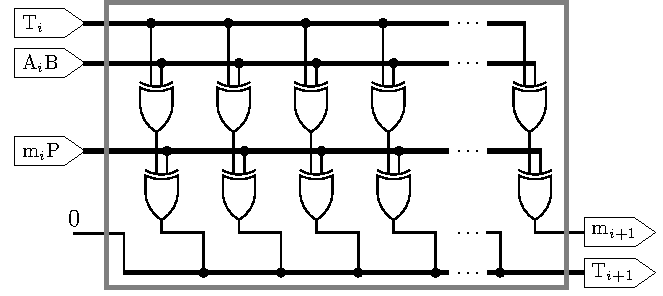
\includegraphics[height=0.5\paperheight]{images/malu-core-basic}
	\end{center}
\end{frame}

\begin{frame}[t]{MALU}
	Modulo Arithmetic Logical Unit [optimized]:\\
	\begin{center}
		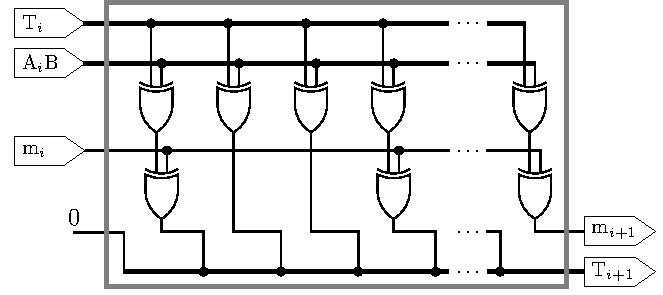
\includegraphics[height=0.5\paperheight]{images/malu-core-optimized}
	\end{center}
\end{frame}


\begin{frame}{Wrappers}
	Multiplication/Addition:\\
	\begin{center}
		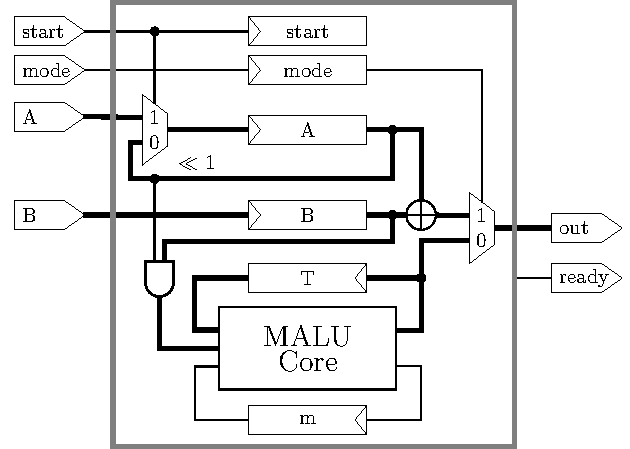
\includegraphics[height=0.55\paperheight]{images/malu-wrapper}
	\end{center}
\end{frame}

\begin{frame}{State of the art}
	Current available implementations:\\
	
	\begin{center}
	\begin{tabular}{lcl}
		Name		&	SW/HW	&	Speed\\
		\hline
		TinyTate	&	SW		&	5s\\
	\end{tabluar}
	\end{center}
\end{frame}

\section{Conclussion}
\subsection*{Conclussion}
\begin{frame}{Progress so far}
	\begin{itemize}
		\item MALU
		\item ECC functions
		\item Pairing functions
	\end{itemize}
\end{frame}

\begin{frame}{To do}
	\begin{itemize}
		\item Bugfixing
		\item Optimization (VHDL)
	\end{itemize}
\end{frame}

\begin{frame}{The end}
	\begin{center}\LARGE Questions?\end{center}
\end{frame}

\end{document}
